\begin{figure}[H]
	\centering
	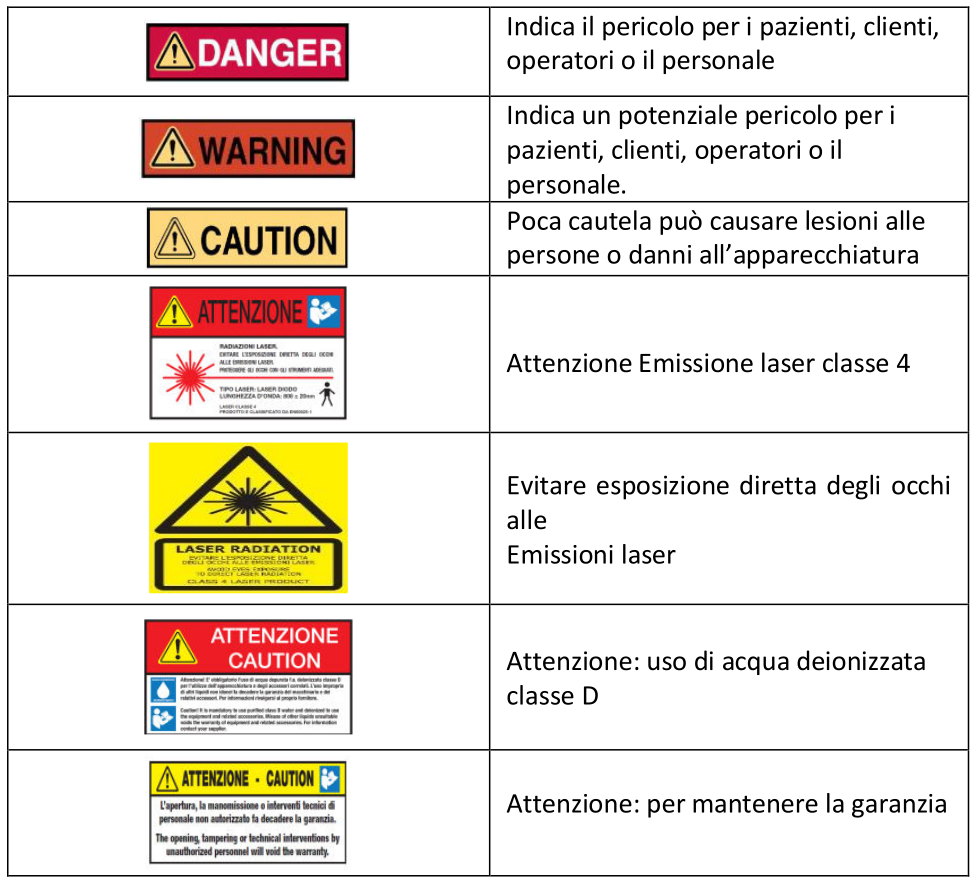
\includegraphics[width=\linewidth]{pittogrammi_1}
%	\caption{}
	\label{fig:pittogrammi1}
\end{figure}
\begin{figure}[H]
	\centering
	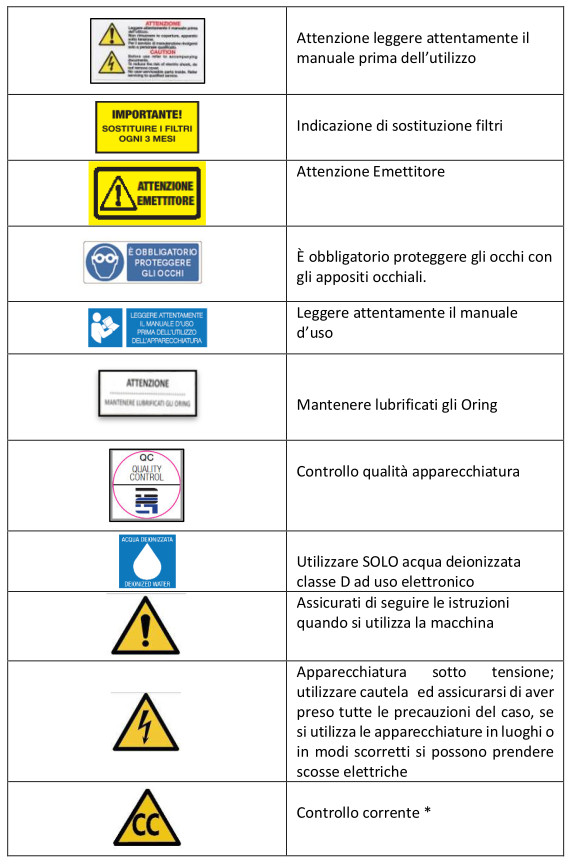
\includegraphics[width=\linewidth]{pittogrammi_2}
%	\caption{}
	\label{fig:pittogrammi2}
\end{figure}
\begin{figure}[H]
	\centering
	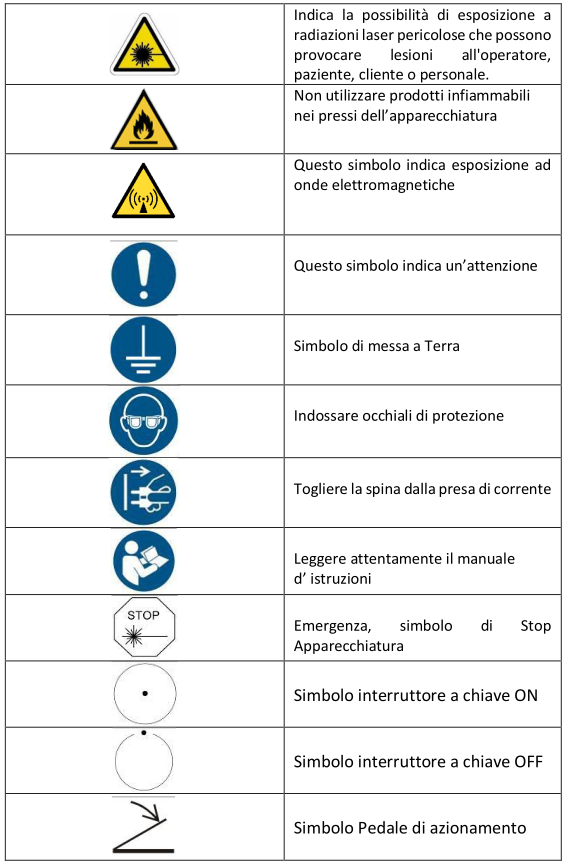
\includegraphics[width=\linewidth]{pittogrammi_3}
%	\caption{}
	\label{fig:pittogrammi3}
\end{figure}
\begin{figure}[H]
	\centering
	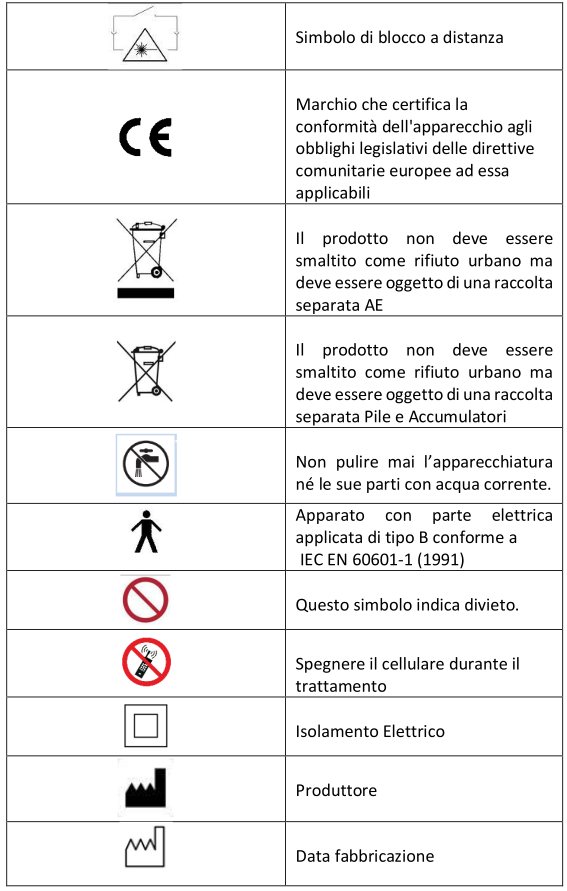
\includegraphics[width=\linewidth]{pittogrammi_4}
%	\caption{}
	\label{fig:pittogrammi4}
\end{figure}
\begin{figure}[H]
	\centering
	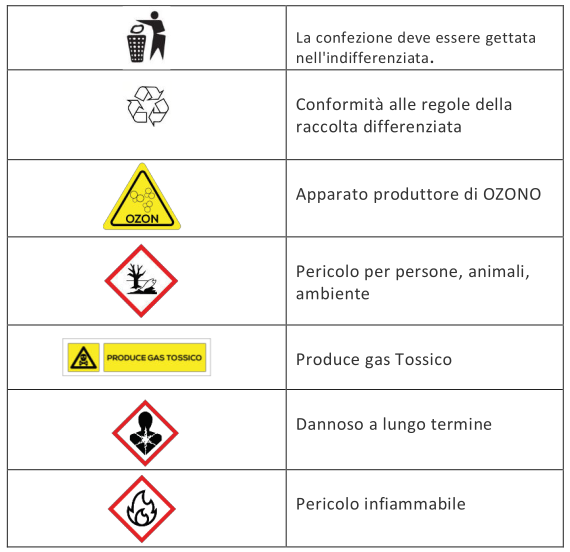
\includegraphics[width=\linewidth]{pittogrammi_5}
%	\caption{}
	\label{fig:pittogrammi5}
\end{figure}
